\documentclass{HustGraduPaper}
%进行个人信息设置
\title{论文题目} %论文题目
\author{作者姓名} %作者姓名
\date{\today} %日期,默认当日
\school{院系名称} %院系名称
\classnum{专业班级} %专业班级
\stunum {U201300000} %学号
\instructor{指导教师姓名} %指导教师姓名

%添加自己要用的其他宏包
\usepackage{xltxtra}
\begin{document}
	%生成标题页
	%如果要改变填写横杠长度,请这样使用:\maketitle[15em]
	\maketitle
	
	%生成声明与授权书页
	%使用方法:\makestatement[保密年数]{empty/true/false}
	%其中:empty为不填;true为保密,请填写保密年数;false为不保密
	\makestatement{empty}
	
	\clearpage %结束上一页
	\pagenumbering{Roman} %摘要页码为大写罗马数字
	
	%填写中文摘要内容和关键字
	\begin{cnabstract}{关键词1;关键词2;关键词3}
		在正文中添加空行可以实现换行功能
		
		摘要内容摘要内容摘要内容摘要内容摘要内容摘要内容摘要内容摘要内容摘要内容摘要内容摘要内容摘要内容摘要内容摘要内容摘要内容摘要内容摘要内容摘要内容摘要内容摘要内容摘要内容摘要内容摘要内容摘要内容摘要内容
		
		摘要内容摘要内容摘要内容摘要内容摘要内容摘要内容摘要内容摘要内容摘要内容摘要内容摘要内容摘要内容摘要内容摘要内容摘要内容摘要内容摘要内容摘要内容摘要内容摘要内容摘要内容摘要内容摘要内容摘要内容摘要内容
	\end{cnabstract}
	%填写英文摘要内容和关键字
	\begin{enabstract}{Key1; Key2; Key3}
		This is abstract. This is abstract. This is abstract. This is abstract. This is abstract. This is abstract. This is abstract. This is abstract. This is abstract. This is abstract. This is abstract. This is abstract. 
		
		This is abstract. This is abstract. This is abstract. This is abstract. This is abstract. This is abstract. This is abstract. This is abstract. This is abstract. This is abstract. This is abstract. This is abstract. 
	\end{enabstract}
	
	%生成目录(自定义的命令)
	%使用方法:\maketoc[nopagenum/pagenum/pagenumtoc]
	%其中:nopagenum指目录没有页码(默认值);pagenum指目录有页码;
	%pagenumtoc指目录有页码,且目录两字出现在目录中
	%请注意在合适的位置放置\pagenumbering{numstyle}使用新的页码
	\maketoc
	
	\clearpage%结束上一页
	\pagenumbering{arabic} %正文页码为阿拉伯数字
	
	%正文内容从这里开始
	\section{第一节 The first Section}
	这是小四号的正文字体,段间距1.5倍
	
	通过空一行实现段落换行,仅仅是回车并不会产生新的段落
	\subsection{第一小节}
	\subsubsection{第一小小节}
	\subsubsection{第二小小节}
	\paragraph{段落}段落具体文章在此段落具体文章在此段落具体文章在此段落具体文章在此段落具体文章在此段落具体文章在此段落具体文章在此段落具体文章在此段落具体文章在此
	\subparagraph{小段落}段落具体文章在此段落具体文章在此段落具体文章在此段落具体文章在此段落具体文章在此段落具体文章在此段落具体文章在此段落具体文章在此
	\subsection{第二小节}
	这是一大段文字这是一大段文字这是一大段文字这是一大段文字这是一大段文字这是一大段文字这是一大段文字这是一大段文字这是一大段文字这是一大段文字这是一大段文字这是一大段文字这是一大段文字这是一大段文字这是一大段文字这是一大段文字这是一大段文字这是一大段文字这是一大段文字这是一大段文字这是一大段文字这是一大段文字这是一大段文字这是一大段文字这是一大段文字这是一大段文字这是一大段文字这是一大段文字这是一大段文字这是一大段文字这是一大段文字这是一大段文字这是一大段文字这是一大段文字这是一大段文字这是一大段文字这是一大段文字这是一大段文字这是一大段文字这是一大段文字这是一大段文字这是一大段文字这是一大段文字这是一大段文字这是一大段文字这是一大段文字这是一大段文字这是一大段文字这是一大段文字这是一大段文字这是一大段文字这是一大段文字这是一大段文字这是一大段文字这是一大段文字这是一大段文字这是一大段文字这是一大段文字这是一大段文字这是一大段文字这是一大段文字这是一大段文字这是一大段文字这是一大段文字这是一大段文字这是一大段文字这是一大段文字这是一大段文字这是一大段文字这是一大段文字这是一大段文字这是一大段文字这是一大段文字这是一大段文字这是一大段文字这是一大段文字这是一大段文字这是一大段文字这是一大段文字这是一大段文字这是一大段文字这是一大段文字这是一大段文字这是一大段文字这是一大段文字这是一大段文字这是一大段文字这是一大段文字这是一大段文字这是一大段文字这是一大段文字这是一大段文字这是一大段文字这是一大段文字这是一大段文字这是一大段文字这是一大段文字这是一大段文字这是一大段文字这是一大段文字这是一大段文字这是一大段文字这是一大段文字这是一大段文字这是一大段文字这是一大段文字这是一大段文字这是一大段文字这是一大段文字这是一大段文字这是一大段文字这是一大段文字这是一大段文字这是一大段文字这是一大段文字这是一大段文字这是一大段文字这是一大段文字这是一大段文字这是一大段文字这是一大段文字这是一大段文字这是一大段文字这是一大段文字这是一大段文字这是一大段文字这是一大段文字这是一大段文字这是一大段文字这是一大段文字这是一大段文字这是一大段文字这是一大段文字这是一大段文字这是一大段文字这是一大段文字这是一大段文字这是一大段文字这是一大段文字
	\section{第二节}
	新的大节会自动出现在新的一页上
	
	请注意目录和参考文献的编译过程
	\section{第三节}
	这是一个引用的范例\cite{Stone_1998}
	
	这样可以添加一个不标注的引用\nocite{9787508342894}
	
	这样可以添加所有bib文件中的参考文献\nocite{*}
	
	在文中引用公式可以这么写:$a^2+b^2=c^2$这是勾股定理,他还可以表示为$c=\sqrt{a^2+b^2}$,还可以让公式单独一段并且加上编号
	\begin{equation}
	sin^2{\theta}+cos^2{\theta}=1 \label{eq:pingfanghe}
	\end{equation}
	还可以通过添加标签在正文中引用公式,如等式~\eqref{eq:pingfanghe}或者\autoref{eq:pingfanghe}。我们还可以轻松打出一个矩阵
	\begin{equation}
	\bm{A}=\begin{bmatrix}
	1&2&3&4\\
	11&22&33&44\\
	\end{bmatrix}
	\times\begin{bmatrix}
	22&24\\
	32&34\\
	42&44\\
	52&54\\
	\end{bmatrix}
	\end{equation}
	或者多个带编号的公式
	\begin{eqnarray}
	f_1(x)=12x^2+36x+sinx\\
	f_2(x)=sqrt[3]{x^3+3x}
	\end{eqnarray}
	以上
	
	\section{用图和表的示例}
	\subsection{图的使用}
	\XeLaTeX 环境下可以使用EPS、PDF、PNG、JPEG、BMP格式的图片,当然也可以用绘图包直接在\LaTeX 中绘制图形,推荐使用宏包tikz。图的环境是figure但figure环境使用复杂,因此本模板定义了一个通用版本的figure,该环境会将figure内的图片居中并设置标签与引用名,同时会让图片位置设置为所有可行位置(htbp,即此处、页顶、页底、独立一页)。
	
	其使用方法如下:
	
	\begin{generalfig}{大数据信息处理框架}{fig:data}
		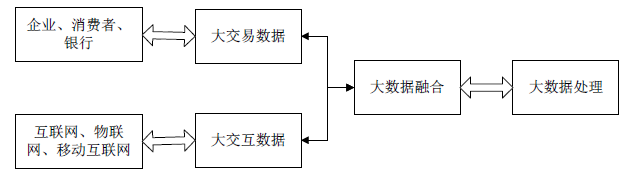
\includegraphics[width=\textwidth]{Figures/data.png}
	\end{generalfig}
	
	同时也可以引用该图片例如:\autoref{fig:data}。请注意generalfig第一个参数是标题,第二个参数是引用。
	
	\newpage
	
	\subsection{表的使用}
	建议使用三线表
	定义了新的做中有
	使用tabularx方便做表
	\begin{generaltab}{某校学生升高体重样本}{tab:heightweight}
		\begin{tabularx}{\textwidth}{lCCC}
			\toprule
			序号&年龄&身高&体重\\
			\midrule
			1&14&156&42\\
			2&16&158&45\\
			3&14&162&48\\
			4&15&163&50\\
			\cmidrule{2-4}
			平均&15&159.75&46.25\\
			\bottomrule
		\end{tabularx}
	\end{generaltab}
	
	啦啦啦
	
	
	\section{测试多页目录的效果}
	wtf
	\subsection{测试多页目录的效果}
	\subsection{测试多页目录的效果}
	\subsection{测试多页目录的效果}
	\subsection{测试多页目录的效果}
	\subsection{测试多页目录的效果}
	\subsection{测试多页目录的效果}
	\subsection{测试多页目录的效果}
	abc
	\section{测试多页目录的效果}
	\subsection{测试多页目录的效果}
	\subsection{测试多页目录的效果}
	\subsection{测试多页目录的效果}
	\subsection{测试多页目录的效果}
	\subsection{测试多页目录的效果}
	\subsection{测试多页目录的效果}
	\subsection{测试多页目录的效果}
	\subsection{测试多页目录的效果}
	whatever
	
	\begin{thankpage}
		感谢老师感谢老师感谢老师感谢老师感谢老师感谢老师感谢老师感谢老师感谢老师感谢老师感谢老师感谢老师感谢老师感谢老师感谢老师感谢老师感谢老师感谢老师感谢老师感谢老师感谢老师感谢老师感谢老师感谢老师感谢老师感谢老师感谢老师感谢老师感谢老师感谢老师感谢老师感谢老师感谢老师感谢老师感谢老师感谢老师
		
		感谢老师感谢老师感谢老师感谢老师感谢老师感谢老师感谢老师感谢老师感谢老师感谢老师感谢老师感谢老师感谢老师感谢老师感谢老师感谢老师感谢老师感谢老师感谢老师感谢老师感谢老师感谢老师感谢老师感谢老师感谢老师感谢老师
	\end{thankpage}
	
	%生成参考文献
	%添加到目录
	\clearpage
	\phantomsection
	\addcontentsline{toc}{section}{参考文献}
	%使用方法:\bibliography{参考文件1文件名, 参考文献2文件名, ...}
	\bibliography{Bibs/mybib}
	
	\begin{appendices}
		\section{这是第一个附录}
		这里是附录环境,其中的section、subsection、subsubsection已经变为附录的样式,并且会以这种样式加入目录中
		\subsection{附录可以有小节}
		\subsubsection{附录中也可以有小小节}
	\end{appendices}
	
\end{document}